\documentclass[tikz]{standalone}
\usepackage{amsmath,amssymb}
\usetikzlibrary{arrows.meta,positioning,calc,decorations.pathreplacing,shapes.geometric}

\begin{document}
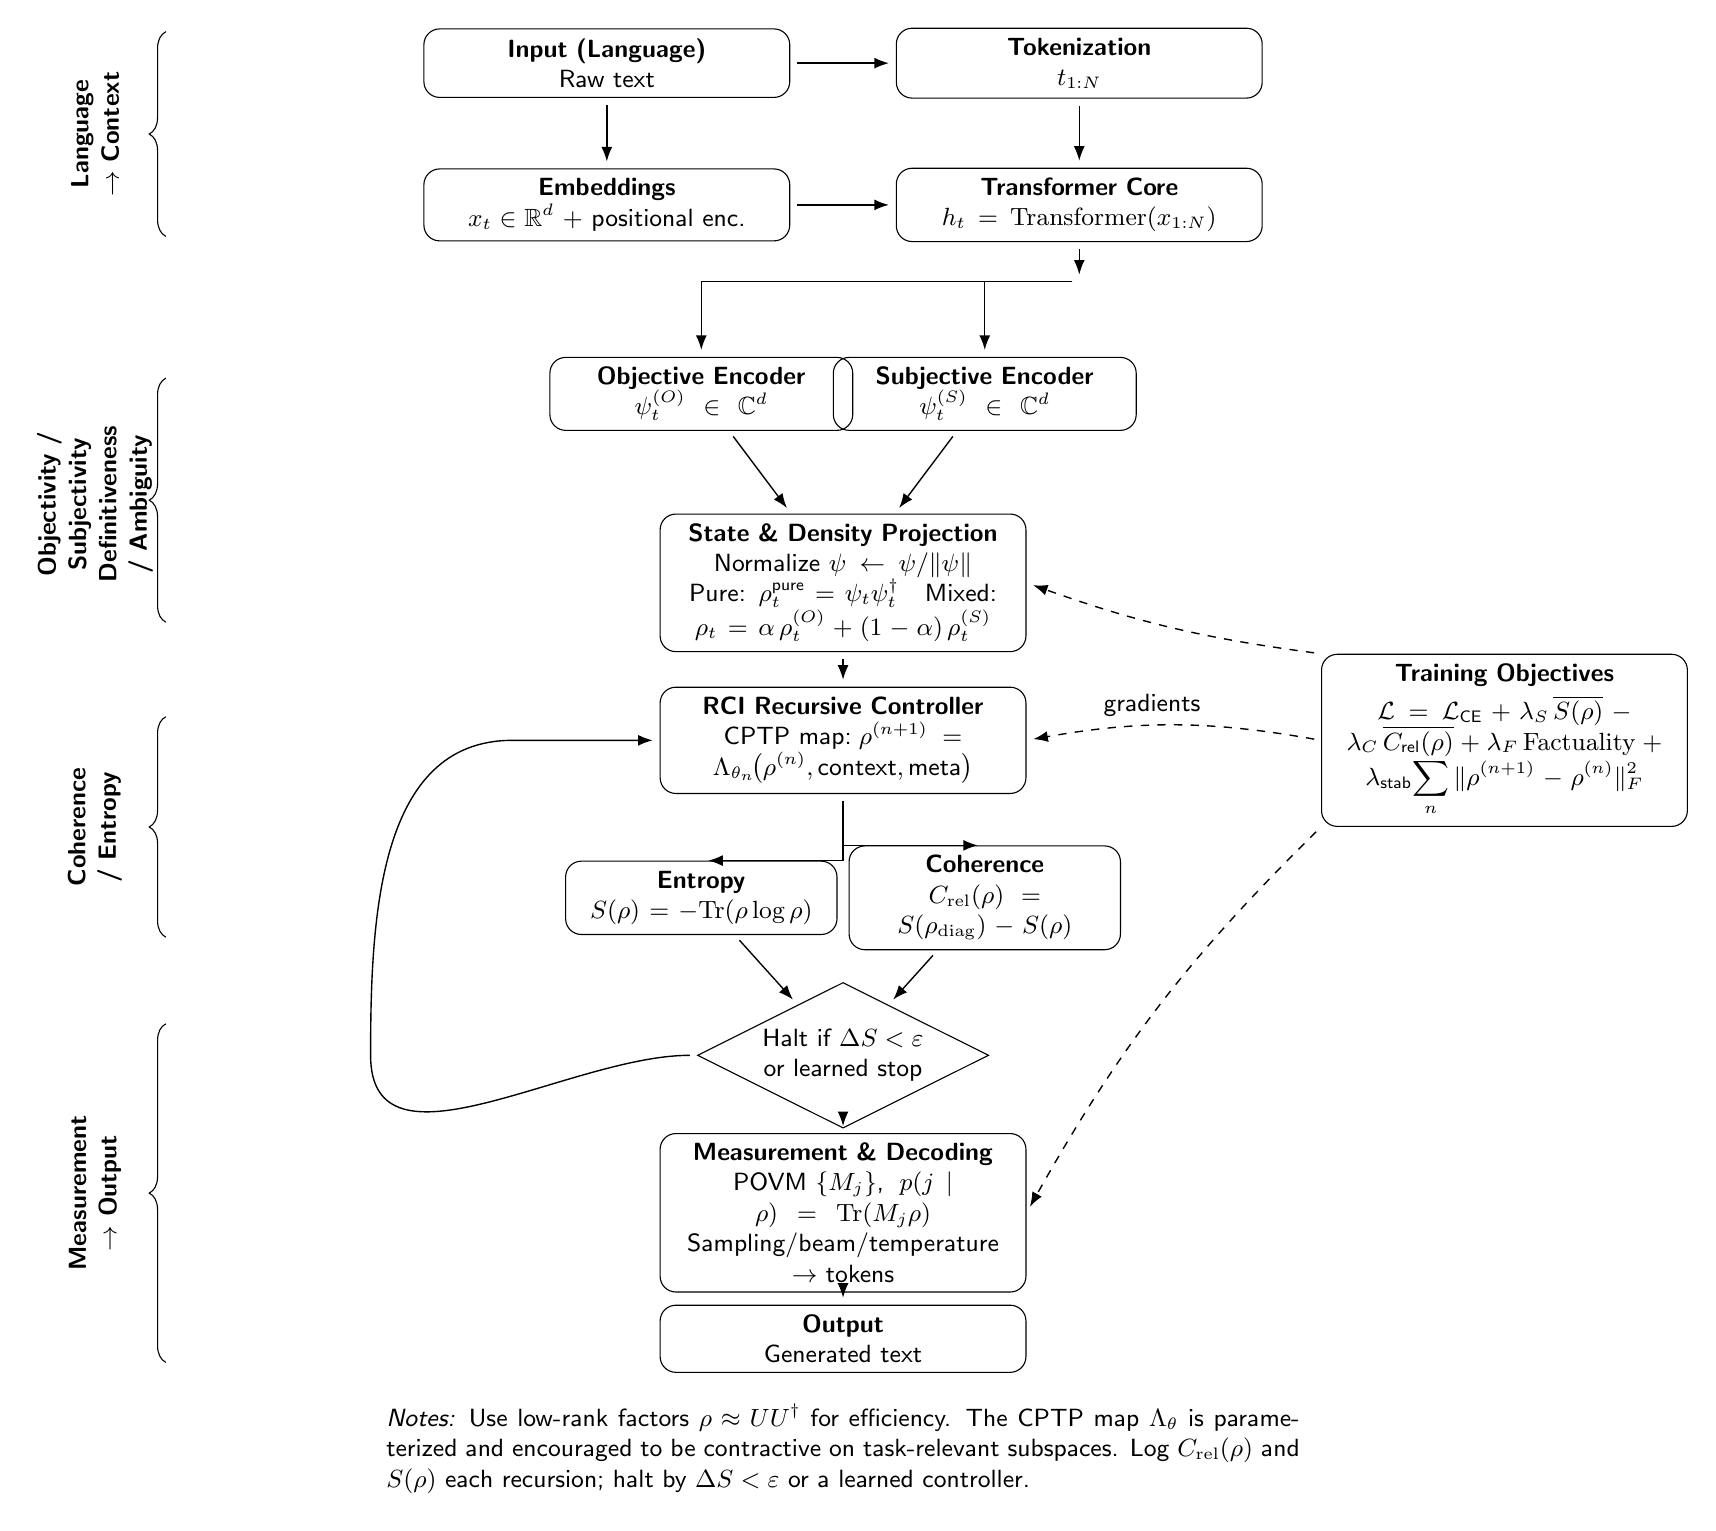
\begin{tikzpicture}[
  font=\sffamily\small,
  >=LaTeX,
  % ---- Node styles ----
  block/.style={draw, rounded corners=2mm, align=center, inner sep=3.5pt,
                minimum height=8mm},
  wide/.style={block, text width=44mm},
  narrow/.style={block, text width=36mm},
  tiny/.style={block, text width=32mm},
  decision/.style={draw, diamond, aspect=2, inner sep=1.5pt, align=center},
  % ---- Lines ----
  line/.style={-Latex, line width=0.5pt, shorten >=2.5pt, shorten <=2.5pt},
  dline/.style={line, dashed},
  % ---- Braces ----
  brace/.style={decorate, decoration={brace, amplitude=6pt}},
  % ---- Vertical label node (for brace text) ----
  vlabel/.style={rotate=90, align=center, text width=24mm}
]

% ===== Fixed coordinates (x in cm, y in cm) =====
% columns: 0 (left), 6 (right), center=3
% rows: 0, -1.8, -4.2, -6.6, -8.6, -10.6, -12.6, -14.6, -16.2

% Row 1
\node[wide]   (input) at (0,   0.0) {\textbf{Input (Language)}\\Raw text};
\node[wide]   (tok)   at (6.0, 0.0) {\textbf{Tokenization}\\$t_{1:N}$};

% Row 2
\node[wide]   (emb)   at (0,  -1.8) {\textbf{Embeddings}\\$x_t\!\in\!\mathbb{R}^d$ + positional enc.};
\node[wide]   (trf)   at (6.0,-1.8) {\textbf{Transformer Core}\\$h_t=\mathrm{Transformer}(x_{1:N})$};

% Row 3
\node[narrow] (obj)   at (1.2,-4.2) {\textbf{Objective Encoder}\\$\psi_t^{(O)}\in\mathbb{C}^d$};
\node[narrow] (subj)  at (4.8,-4.2) {\textbf{Subjective Encoder}\\$\psi_t^{(S)}\in\mathbb{C}^d$};

% Row 4 (centered)
\node[wide]   (rho)   at (3.0,-6.6) {\textbf{State \& Density Projection}\\
  Normalize $\psi\leftarrow \psi/\|\psi\|$\\
  Pure: $\rho^{\text{pure}}_t=\psi_t\psi_t^\dagger$\quad
  Mixed: $\rho_t=\alpha\,\rho_t^{(O)}+(1-\alpha)\,\rho_t^{(S)}$
};

% Row 5
\node[wide]   (rci)   at (3.0,-8.6) {\textbf{RCI Recursive Controller}\\
  CPTP map:\;$\rho^{(n+1)}=\Lambda_{\theta_n}\!\big(\rho^{(n)},\text{context},\text{meta}\big)$
};

% Row 6 (symmetric)
\node[tiny]   (entropy) at (1.2,-10.6) {\textbf{Entropy}\\$S(\rho)=-\mathrm{Tr}(\rho\log\rho)$};
\node[tiny]   (coh)     at (4.8,-10.6) {\textbf{Coherence}\\$C_{\mathrm{rel}}(\rho)=S(\rho_{\mathrm{diag}})-S(\rho)$};

% Row 7
\node[decision] (halt) at (3.0,-12.6) {Halt if $\Delta S<\varepsilon$\\or learned stop};

% Row 8
\node[wide]   (meas)  at (3.0,-14.6) {\textbf{Measurement \& Decoding}\\
  POVM $\{M_j\}$,\; $p(j\!\mid\!\rho)=\mathrm{Tr}(M_j\rho)$\\
  Sampling/beam/temperature $\rightarrow$ tokens
};

% Row 9
\node[wide]   (out)   at (3.0,-16.2) {\textbf{Output}\\Generated text};

% Side: Loss block
\node[wide]   (loss)  at (11.4,-8.6) {\textbf{Training Objectives}\\[1mm]
$\displaystyle \mathcal{L}=\mathcal{L}_{\text{CE}}
+ \lambda_S\,\overline{S(\rho)}
- \lambda_C\,\overline{C_{\text{rel}}(\rho)}
+ \lambda_F\,\mathrm{Factuality}
+ \lambda_{\text{stab}}\!\sum_n\|\rho^{(n+1)}-\rho^{(n)}\|_F^2$};

% ===== Connections =====
\draw[line] (input) -- (tok);
\draw[line] (input) -- (emb);
\draw[line] (tok)   -- (trf);
\draw[line] (emb)   -- (trf);

% neat fan-out: down from trf, split to encoders
\path (trf.south) ++(0,-0.5) coordinate (splitA);
\draw[line] (trf.south) -- (splitA);
\draw[line] (splitA) -| (obj.north);
\draw[line] (splitA) -| (subj.north);

\draw[line] (obj) -- (rho);
\draw[line] (subj) -- (rho);

\draw[line] (rho) -- (rci);
\draw[line] (rci) |- (entropy.north);
\draw[line] (rci) |- (coh.north);

\draw[line] (entropy) -- (halt);
\draw[line] (coh)     -- (halt);

\draw[line] (halt) -- (meas);
\draw[line] (meas) -- (out);

% feedback loop: outside on the far left margin
\path (-3.0,-12.6) coordinate (Lturn);
\draw[line] (halt.west) to[out=180,in=-90] (Lturn)
           to[out=90,in=180]  (-1.2,-8.6)
           -- ++(0.6,0) -- (rci.west);

% dashed training edges (clear of nodes)
\path[dline] (loss.west) edge[bend right=10] node[above,pos=0.58]{gradients} (rci.east);
\path[dline] (loss.north west) edge[bend left=6] (rho.east);
\path[dline] (loss.south west) edge[bend right=8] (meas.east);

% ===== Stage braces + labels (moved farther left, fixed width) =====
% Brace column farther left:
\def\BXL{-5.6}
% Language -> Context
\draw[brace] (\BXL,-2.2) -- (\BXL,0.4);
\node[vlabel] at (\BXL-0.9,-0.9) {\textbf{Language $\to$ Context}};

% Objectivity/Subjectivity + Definitiveness/Ambiguity
\draw[brace] (\BXL,-7.1) -- (\BXL,-4.0);
\node[vlabel] at (\BXL-0.9,-5.6) {\textbf{Objectivity / Subjectivity}\\\textbf{Definitiveness / Ambiguity}};

% Coherence / Entropy
\draw[brace] (\BXL,-11.1) -- (\BXL,-8.3);
\node[vlabel] at (\BXL-0.9,-9.7) {\textbf{Coherence / Entropy}};

% Measurement -> Output
\draw[brace] (\BXL,-16.5) -- (\BXL,-12.2);
\node[vlabel] at (\BXL-0.9,-14.35) {\textbf{Measurement $\to$ Output}};

% ===== Footnote =====
\node[align=left] at (3.0,-17.6) {\begin{minipage}{11.6cm}
\textit{Notes:} Use low-rank factors $\rho\approx UU^\dagger$ for efficiency. The CPTP map $\Lambda_\theta$
is parameterized and encouraged to be contractive on task-relevant subspaces. Log $C_{\mathrm{rel}}(\rho)$
and $S(\rho)$ each recursion; halt by $\Delta S<\varepsilon$ or a learned controller.
\end{minipage}};

\end{tikzpicture}
\end{document}

